\documentclass[a4paper, 11pt]{article}

\usepackage{amsmath}
\usepackage{amssymb}
\usepackage{hyperref}
\usepackage{makeidx}
\usepackage{graphicx}
\usepackage{titlesec}
\titlespacing{\section}{0pt}{\parskip}{-\parskip}
\titlespacing{\subsection}{0pt}{\parskip}{-\parskip}
\graphicspath{{figures/}} % Directory in which figures are stored
\usepackage{natbib}% \bibliography
\usepackage{float}
\usepackage{setspace} % for line spacing
\usepackage[margin=1in]{geometry}
\title{Assignment3 Clustering-CSE780}
\author{Paria, Fakhrzad \\ Stuent ID: 400353290 }
\date{7-Nov-2021}
\setstretch{1.3}
\setlength\abovecaptionskip{-5pt}

\begin{document}
	
	\maketitle
	\newpage
\section*{Part a.Data Summary}
In this project we will use a dataset related to an insurance company ~\cite{data}. There are 10000 customer in this data. Also there is 18features that one of them is a label, a factor variable that shows whether customer had insurance claim last year or not. The correlation between variables shows in figure1.\newline
There are 1939 $NA$ values in dataset that all have removed. And since we need to perform distance and scale functions just below 15 numeric features select for this clustering. Also the last column that is label has been omitted.\newline
$X1$ age    -            Min:20  Max:65  Mean:42 \newline
$X2$ gender -            female: 4084(50\%)   male: 4065(50\%) \newline
$X3$ race   - majority(0): 7323(90\%)  minority(1): 826(10\%)\newline
$X4$ driving experience - Min:5   Max:35   Mean:16 \newline
$X5$ education - none(1): 1528(19\%)   high school(2):3404(42\%)  university(3):3217(39\%)\newline
$X6$ income - upper(1):3588(44\%) middle(2): 1727(21\%) working(3):1375(17\%) poverty(4):1459(18\%) \newline
$X7$ Credit score -     Min:0.0533   Max:0.960  Mean:0.516 \newline
$X8$ vehicle ownership  True(1):5698(70\%)   False(0): 2451(30\%) \newline
$X9$ married-           True(1): 4083(50\%)  False(0): 4066(50\%) \newline
$X10$ children          True(1): 5617(69\%)  False(0): 2532(31\%) \newline
$X11$ postal code- this is 5 different code and it has meaning based on company definition\newline
$X12$ annual mileage-     Min:2000    Max: 22000   Mean: 11693 \newline
$X13$ speeding violation- Min:0       Max:22       Mean: 1.48  \newline
$X14$ DUI -               Min:0       Max:6        Mean: .25 \newline
$X15$ past accident -     Min:0       Max:15       Mean: 1\newline
We can see that customers with average age 20 and income level poverty and education level high school have more accident claim in last year. 
\begin{figure}[H]
	\centering
	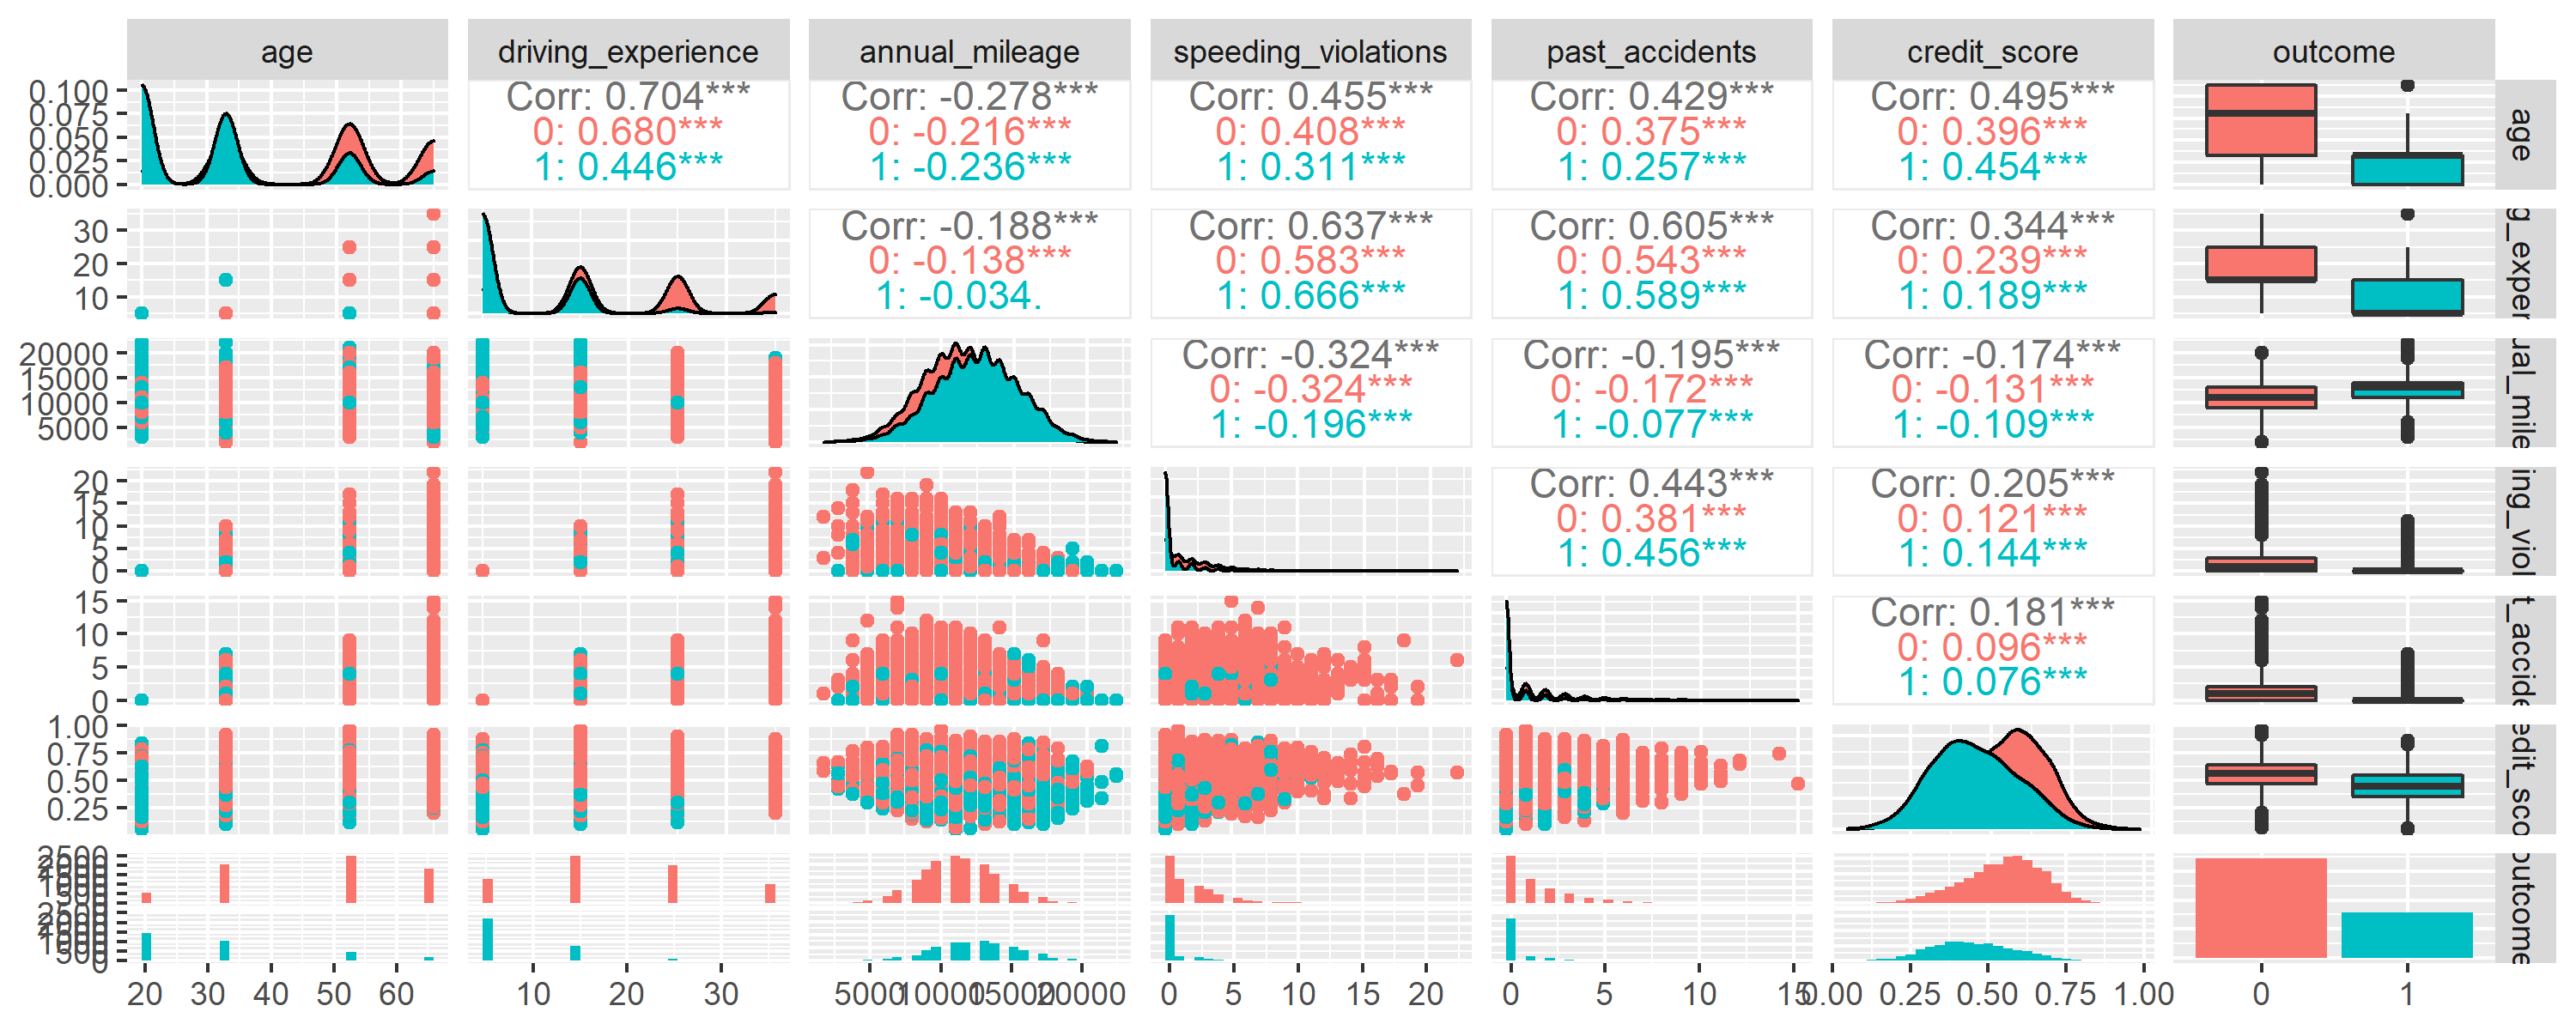
\includegraphics[width=\textwidth]{figure1.png}
	\caption{Features relationship}
\end{figure}

\section*{Part b.Clustering}
In This part we use three clustering algorithm, Kmeans, Hierarchical and Gaussian Mixture model and the goal is finding the best clusters of customers that show same pattern based on this dataset features. For preparing the dataset, we normalize all columns also calculate the distance matrix by euclidean method. 
\subsection*{b.1 K-means Clustering}
First of all we need to  know optimal number of clusters and there are two method for calculating this K. it shows in figure2 that is 2.
\begin{figure}[H]
	\centering
	\begin{minipage}[b]{.7\textwidth}
		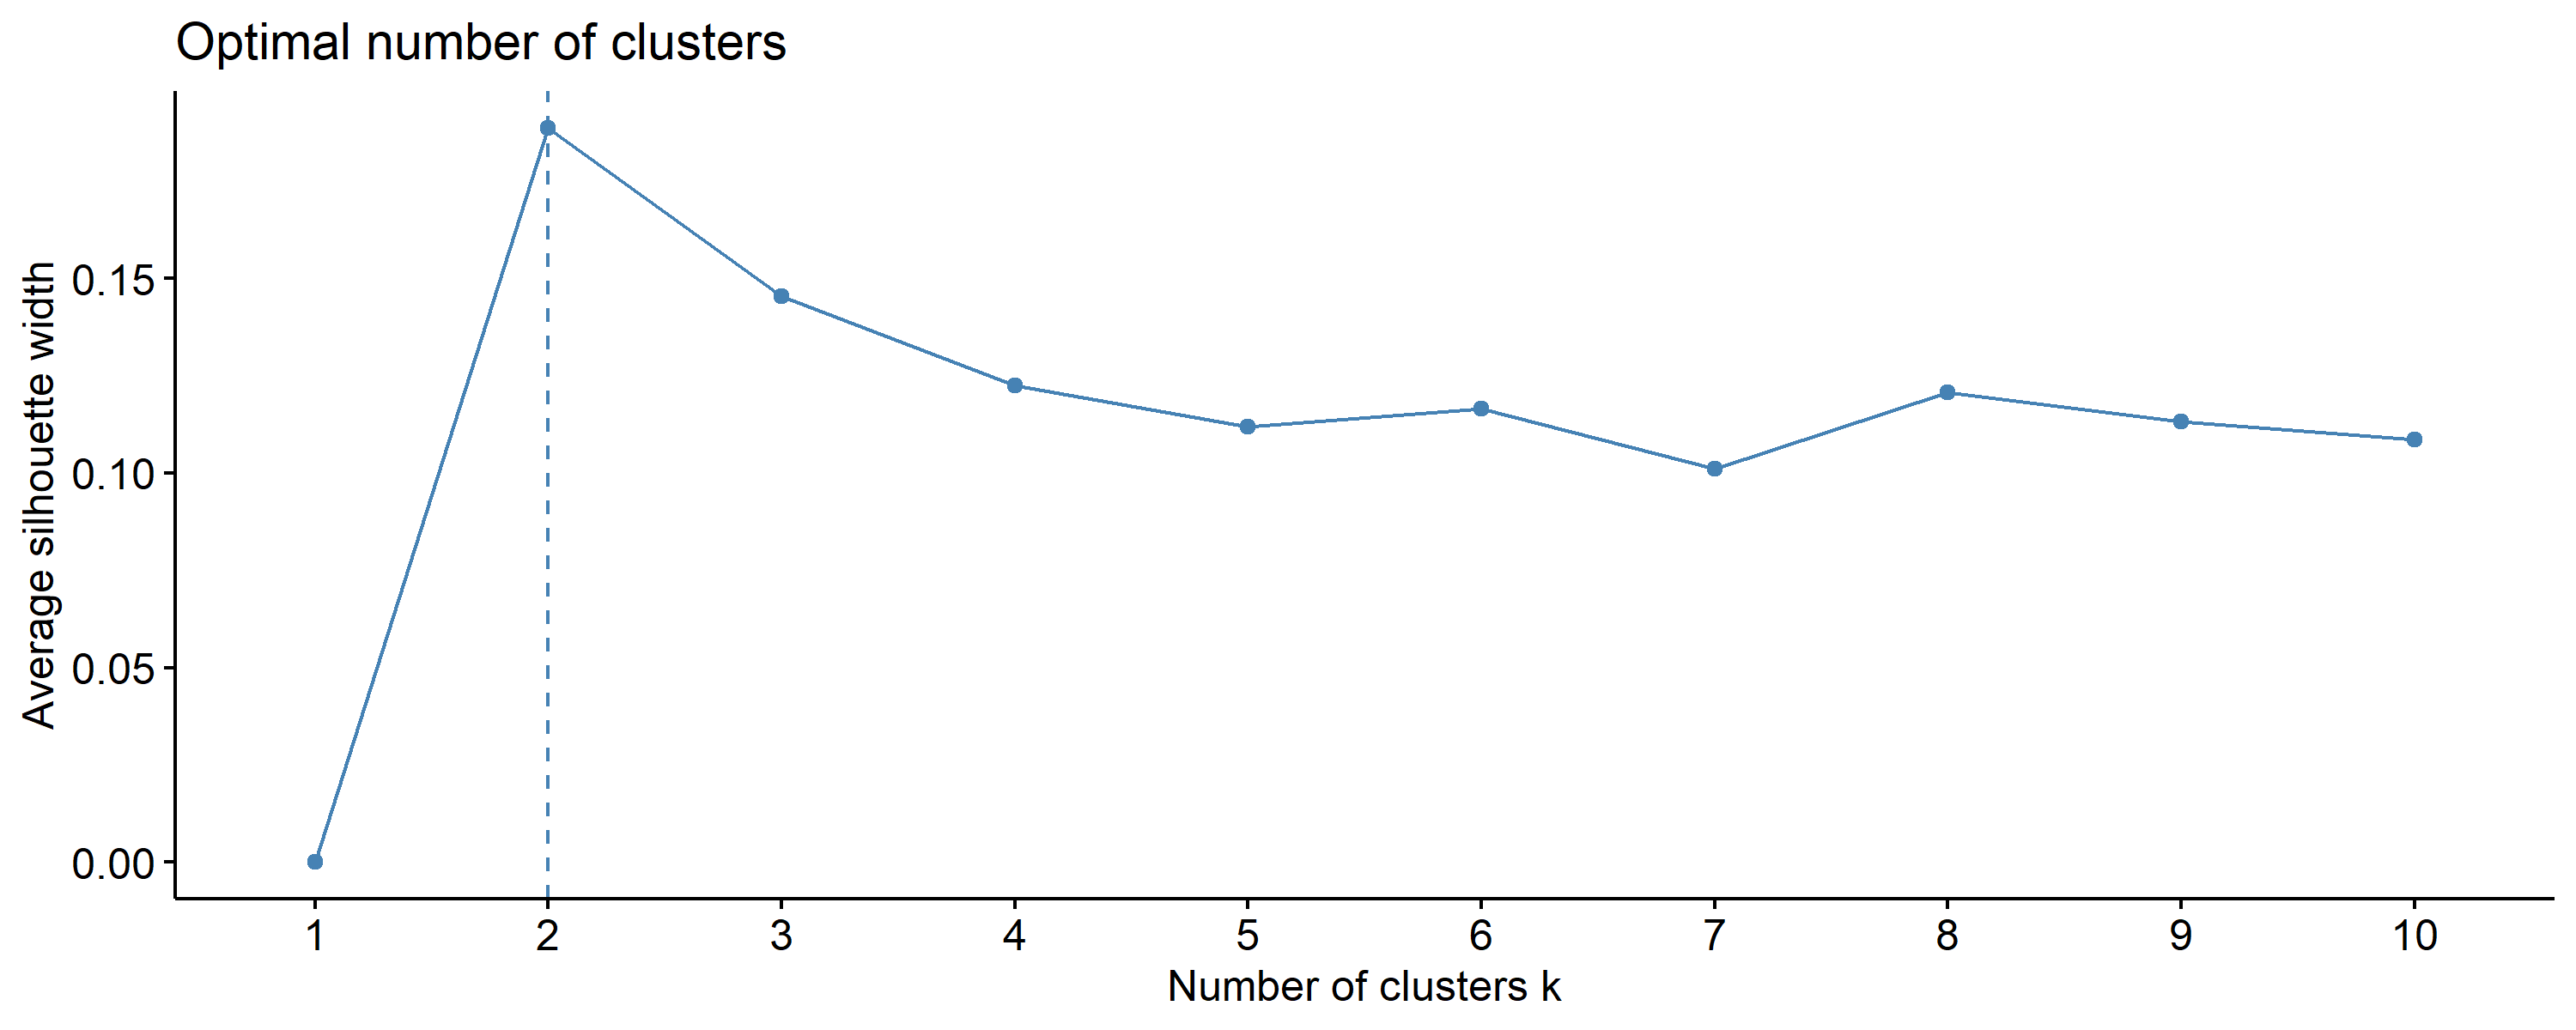
\includegraphics[width=\textwidth]{figure17.png}
		\caption{silhouette}
	\end{minipage}
\end{figure}
After fitting K-mean we see that the $Within cluster sum of squares by cluster$ are 57355.83 and 39454.42 respectively and (between\_SS / total\_SS =  20.8\%).Figure3 shows these clusters based on two features credit\_score and annual\_milleage.
\subsection*{b.2 Hierarchical Clustering}
In this part we fit hierarchical model with four linkage $single$, $complete$,$average$ and $centroid$. Since the number of customers are huge the dendogram plots are not clear and here we cut it by 2.

\subsection*{b.3 Gaussian Mixture Model clustering}
As we can see  in figure 4 and 5 the hierarchical and Gaussion models don't perform well in this dataset when the number of observations are huge and we need 2 clusters.

\begin{figure}[H]
	\centering
	\begin{minipage}[b]{.4\textwidth}
		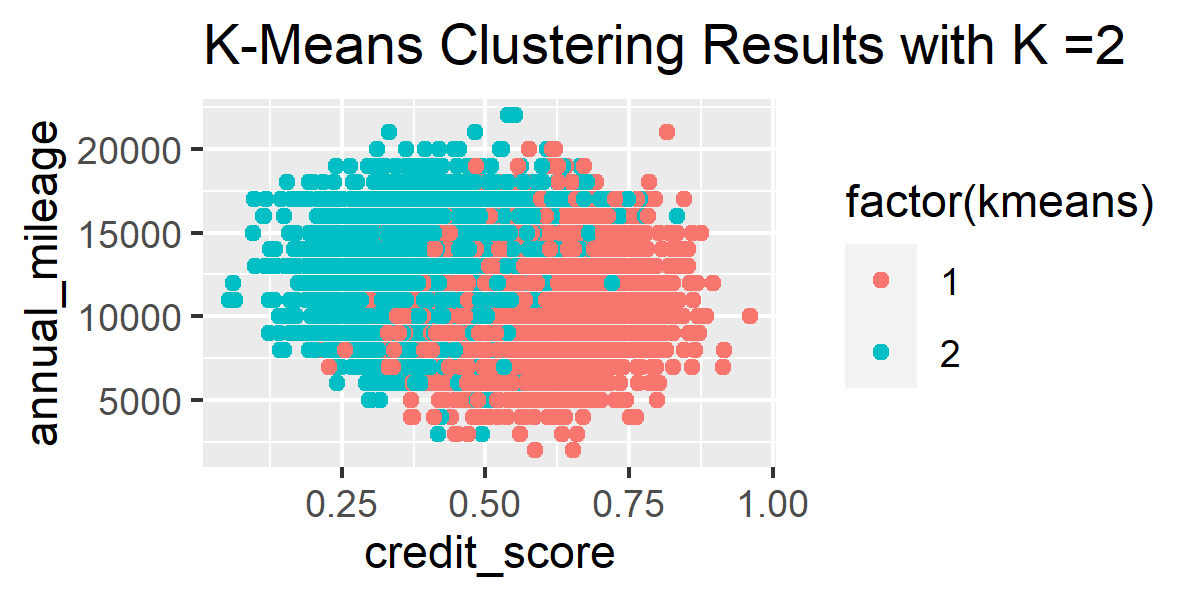
\includegraphics[width=\textwidth]{figure6.png}
		\caption{K-means}
	\end{minipage}
 \hfill
	\begin{minipage}[b]{.4\textwidth}
	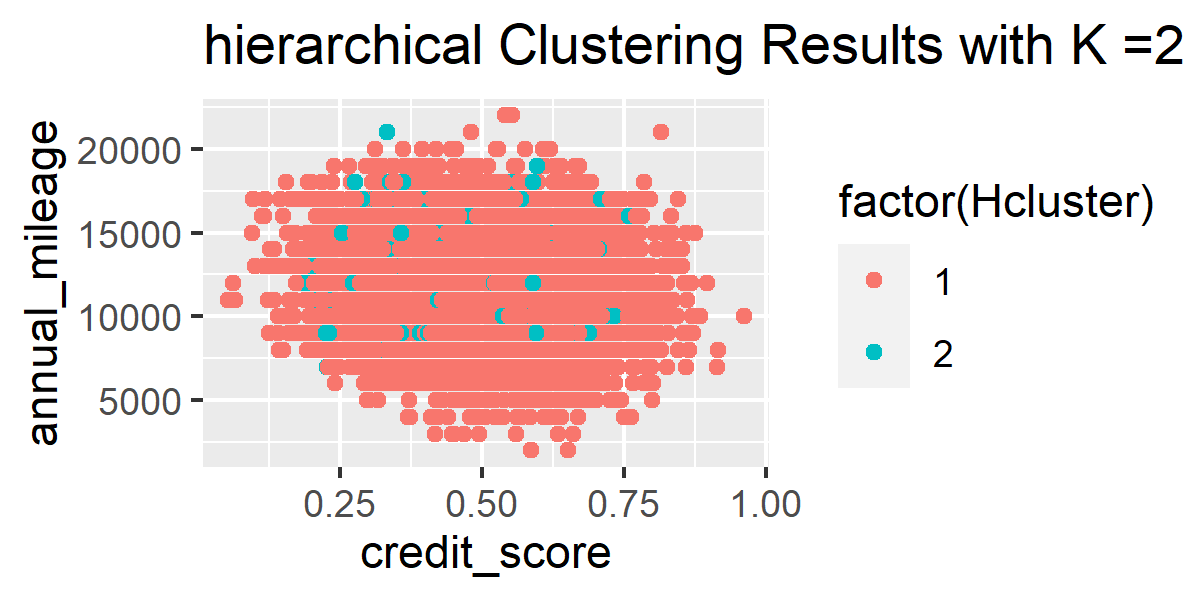
\includegraphics[width=\textwidth]{figure11.png}
	\caption{Hierarchical}
\end{minipage}
\hfill
\begin{minipage}[b]{.4\textwidth}
	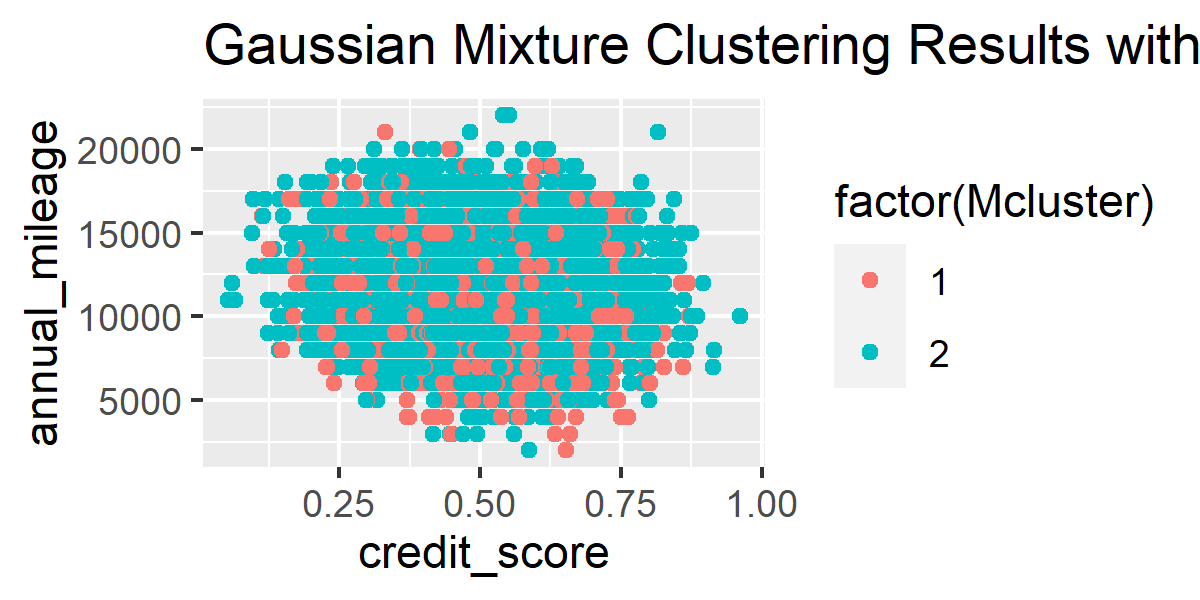
\includegraphics[width=\textwidth]{figure12.png}
	\caption{Gaussian Mixture Model}
\end{minipage}
\hfill
\begin{minipage}[b]{.4\textwidth}
	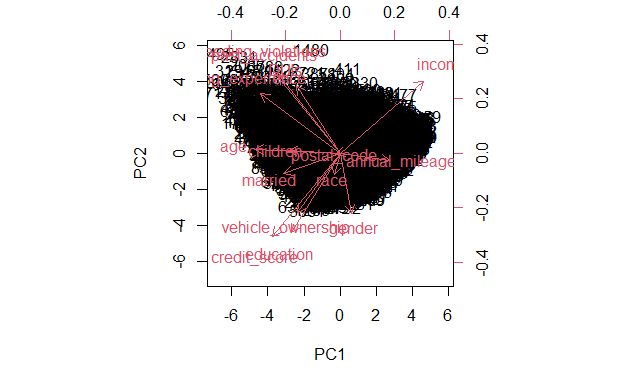
\includegraphics[width=\textwidth]{figure20.png}
	\caption{PCA Variance }
\end{minipage}
\end{figure}
\section*{c.Principal Component Analysis}	
In this Part we used PCA for dimension reduction to see the effect on the result of clustering models.
\subsection*{c.1  Perform PCA}
When we perform PCA, see that 15 PCA will be generate that the details are in table1.
\begin{table}[ht]
	\centering
			\caption{PCA}
	\label{table1}
	\begin{tabular}{crrrrrrrrr}
		\hline
		& PC1 & PC2 & PC3 & PC4 & PC5 & PC6 & PC7 & PC8 & PC9  \\ 
		\hline
		Standard deviation & 2.1037 & 1.2785 & 1.1614 & 1.0429 & 1.0209 & 0.9884 & 0.8856 & 0.8644 & 0.8345  \\ 
		Proportion of Variance & 0.2950 & 0.1090 & 0.0899 & 0.0725 & 0.0695 & 0.0651 & 0.0523 & 0.0498 & 0.0464  \\ 
		Cumulative Proportion & 0.2950 & 0.4040 & 0.4939 & 0.5664 & 0.6359 & 0.7010 & 0.7533 & 0.8031 & 0.8496 \\ 
		\hline
	\end{tabular}
\end{table}
\begin{table}[ht]
	\centering
	\begin{tabular}{crrrrrr}
		\hline
		& PC10 & PC11 & PC12 & PC13 & PC14 & PC15 \\ 
		\hline
		Standard deviation & 0.7565 & 0.7138 & 0.6776 & 0.5931 & 0.4458 & 0.4064 \\ 
		Proportion of Variance & 0.0382 & 0.0340 & 0.0306 & 0.0234 & 0.0132 & 0.0110 \\ 
		Cumulative Proportion & 0.8877 & 0.9217 & 0.9523 & 0.9757 & 0.9890 & 1.0000 \\ 
		\hline
	\end{tabular}
\end{table}
Here we can see that PCA1 and PCA2 have 40\% of variation. In rotation matrix we can see that score of 15 features for PCA1 is not equal and some of features such as `gender`, `race` and `postal\_code` have not explained by PC1, on the other hand PC4 for these features has the most score, see figure6.
\subsection*{c.2 Clustering with PCA }
We fit K-means and hierarchical clustering models by PCA features and see the result in figure 7 and 8.
Since there are less correlation between features and PCA1 and PCA2 just have 40\% of variance, using the PCA reduction is not a good solution in this dataset. 
\begin{figure}[H]
	\centering
	\begin{minipage}[b]{.4\textwidth}
		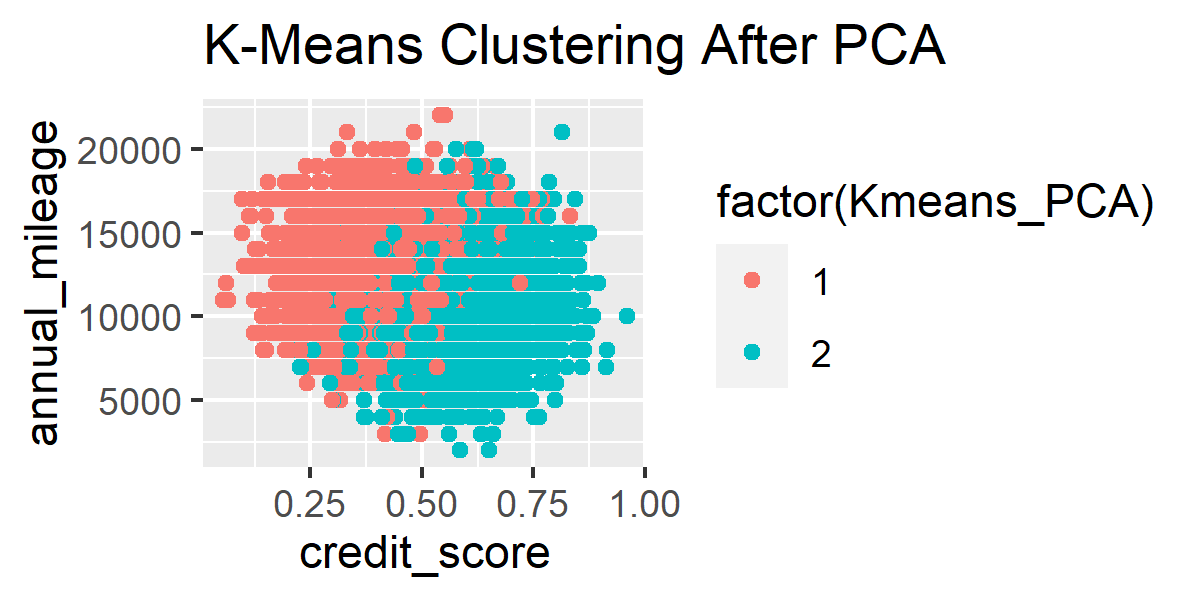
\includegraphics[width=\textwidth]{figure21.png}
		\caption{K-means after PCA}
	\end{minipage}
	\hfill
	\begin{minipage}[b]{.4\textwidth}
		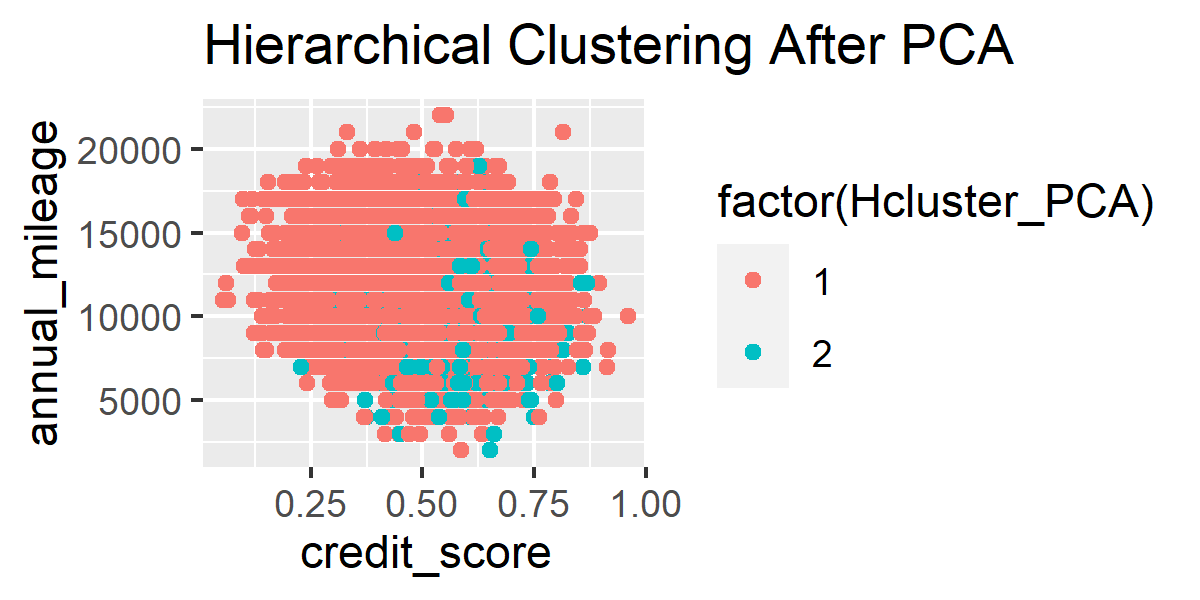
\includegraphics[width=\textwidth]{figure22.png}
		\caption{Hierarchical After PCA}
	\end{minipage}
	\hfill
\begin{minipage}[b]{.4\textwidth}
	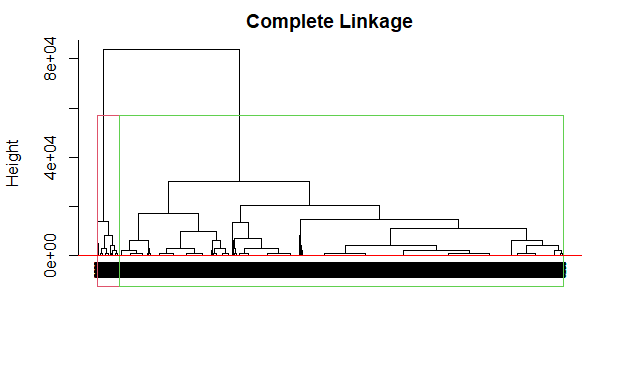
\includegraphics[width=\textwidth]{figure7.png}
	\caption{}
\end{minipage}
	\hfill
\begin{minipage}[b]{.4\textwidth}
	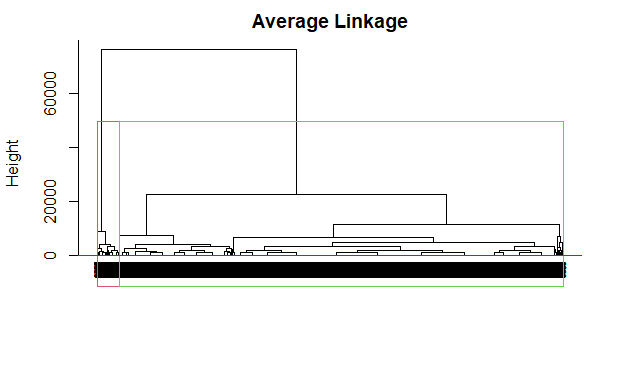
\includegraphics[width=\textwidth]{figure8.png}
	\caption{}
\end{minipage}
	\hfill
\begin{minipage}[b]{.4\textwidth}
	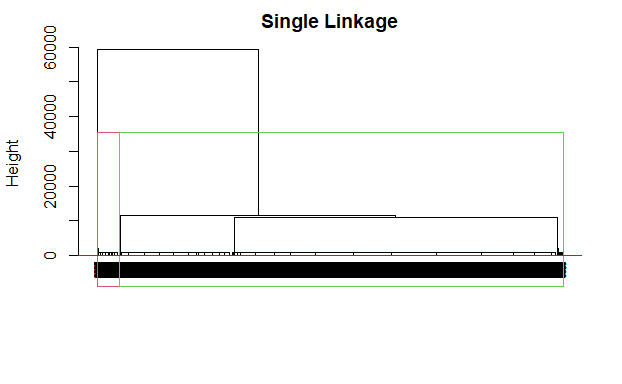
\includegraphics[width=\textwidth]{figure9.png}
	\caption{}
\end{minipage}
	\hfill
\begin{minipage}[b]{.4\textwidth}
	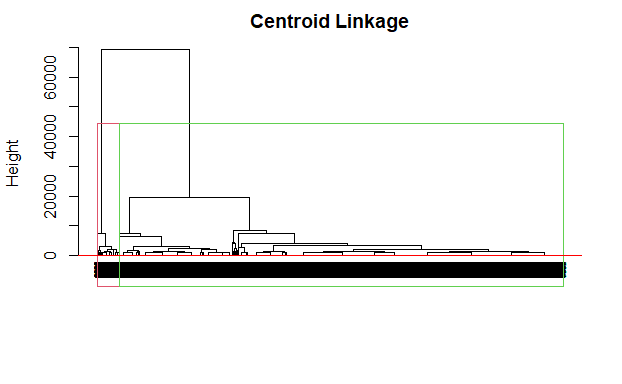
\includegraphics[width=\textwidth]{figure10.png}
	\caption{}
\end{minipage}
\end{figure}
\newpage
\bibliographystyle{plain}
\bibliography{Assignment3}
\end{document}